\chapter{Introduction}
\label{chapter:intro}
When developing a web application, there are numerous issues the application writer must consider. One of the most used languages when designing the front-end of a web application is JavaScript~\cite{javascript_popularity}, a dynamically typed, multi-paradigm programming language~\cite{javascript_info}. Unfortunately, JavaScript suffers from a couple of drawbacks and attacks towards the language through Cross-Site Scripting (XSS) were on the third place on the OWASP Top 10 in 2013.\cite{owasp_xss_rank} In a XSS attack, the attacker manages to inject JavaScript code into websites that are considered secure~\cite{owasp_xss, excess_xss}. These injections can do anything from harmless pranks (e.g. showing an alert box) to redirecting the non-suspecting user to a fake website to steal valuable information. When an attack like XSS succeeds, the culprit is usually non-escaped input from the users. If a website directly includes the user input, an attacker can insert input that will be treated as code by the victim~\cite{excess_xss}. Examples of valuable information retained by the browser for an attacker are cookies and session tokens.
\section{Problems with JavaScript}
From a security standpoint with regards to information-flow control, JavaScript suffers from two big problems, namely
\begin{itemize}
  \item It is weak, dynamically typed.
  \item It can gain access to sensitive information from the browser.
\end{itemize}
There are more problems with JavaScript in general, e.g. bad scoping semantics, poor support for the functional paradigm and a lack of modularity. Since those problems are not that important from a information-flow security standpoint, it will not be looked at in this report. The curious reader can read more about those problems in~\cite{haste-lang}.

\section{Information-Flow Control}
Confidentiality in any system is important. Unfortunately, there are few built in mechanisms for ensuring end-to-end confidentiality policies~\cite{ifc-jsac}. The general idea behind information flow control is to tag the data with one of two security levels; \emph{high} or \emph{low}. These levels can be seen as either private data (high security level) or public data (low security level). Figure~\ref{fig:normal_flow} shows the flow in an application developed with the core language of JavaScript. In JavaScript, there is no way of controlling the flow by dividing the different values of the application into either a high or low context. It is more of a straight line from the input to the output. However, if an implementation of a system that enforces information-flow control were in place, the flow could be seen as in Figure~\ref{fig:controlled_flow}. The only flow that is not allowed is a flow from a high context to a low context. All the other flows, i.e. low to low, low to high and high to high, are valid. A system that enforces information-flow control will help in ensuring end-to-end confidentiality.
\begin{figure}[h]
  \begin{subfigure}{.5\textwidth}
    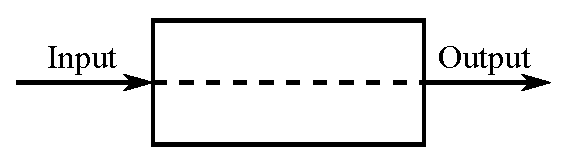
\includegraphics[scale=0.65]{images/flow_normal.eps}
    \caption{Normal information flow}
    \label{fig:normal_flow}
  \end{subfigure}
  \begin{subfigure}{.5\textwidth}
    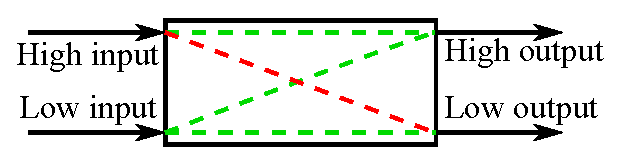
\includegraphics[scale=0.65]{images/flow_controlled.eps}
    \caption{Controlled information flow}
    \label{fig:controlled_flow}
  \end{subfigure}
  \caption{Different kinds of flow in a web application}
  \label{fig:flows}
\end{figure}
